%% ---------------------------------------------------------------------------
%% This file is part of the "Flawed Egyptology" talk.
%%
%% Copyright 2014 by Eugen Wintersberger <eugen.wintersberger@gmail.com>
%%
%% This work is licensed under the Creative Commons
%% Attribution-NonCommercial-ShareAlike 4.0 International License. To view 
%% a copy of this license, visit 
%% http://creativecommons.org/licenses/by-nc-sa/4.0/.
%% ---------------------------------------------------------------------------
\documentclass{beamer}
\usepackage{tikz}
\usepackage{pgfpages}
\usepackage{todonotes}
\usepackage{array}
\usepackage{multirow}
\usepackage{hyperref}
\usepackage{copyrightbox}
\usepackage{minted}
\usepgflibrary{shapes.multipart}
\usepgflibrary{shapes.symbols}
\usetikzlibrary{positioning}
\usetikzlibrary{calc}
\usetikzlibrary{fit}
\usetikzlibrary{datavisualization}


\setbeamercolor{frametitle}{fg=black,bg=white}
\setbeamerfont{frametitle}{series=\bfseries}
\setbeamercolor{part page}{fg=black,bg=white}
\setbeamerfont{part page}{series=\bfseries}
\setbeamercolor{part title}{fg=black}
\setbeamercolor{part subtitle}{fg=black}
\setbeamercolor{author}{fg=white}
\setbeamercolor{date}{fg=white}



\setbeamercolor{title}{fg=black}
\setbeamerfont{title}{series=\bfseries,size=\Huge}
\setbeamercolor{subtitle}{fg=black}

\setbeamercolor{item}{fg=black}


%\setbeameroption{show notes on second screen}

\title{{\Huge Expression Templates}}
\subtitle{Making expressions iterable}
\author{Eugen Wintersberger\\ \small{eugen.wintersberger@gmail.com}}
\date{June 24, 2015}

\begin{document}

\frame{\titlepage}

%%%===========================================================================
\begin{frame}[fragile]{Motivation - why operators}
    In math we have 
    \begin{align}
        I_{\mathrm{corrected}}=\frac{s\left(I-I_{\mathrm{background}}\right)}
                                   {\tau_{\mathrm{exposure}}}
                                   \nonumber
    \end{align}

    \vspace{0.05\textheight}
    In Fortran we could have something like this
    \begin{minted}[fontsize=\small]{fortran}
real(kind=8),dimension(:),allocatable := intensity
real(kind=8),dimension(:),allocatable := corr_intensity
real(kind=8),dimension(:),allocatable := bg
real(kind=8) := exp_time,s

corr_intensity = s*(intensity-bg)/exp_time
    \end{minted}
   
    \vspace{0.05\textheight}
    Code looks quite similar to the formuls written on paper $\Rightarrow$
    less errors!
\end{frame}

%%%---------------------------------------------------------------------------
\begin{frame}[fragile]{The \texttt{C}-version}
In plain \texttt{C}/\texttt{C++} we have to loop

\vspace{0.05\textheight}
\begin{minted}{cpp}
typedef std::vector<doubel> array_type;

array_type intensity,corr_intensity,bg;
double exp_time,s;

for(size_t i=0;i<intensity.size();i++)
    corr_intensity[i]=s*(intensity[i]-bg[i])/exp_time;
\end{minted}

\vspace{0.05\textheight}
Not very elegant.
\end{frame}

%%%---------------------------------------------------------------------------
\begin{frame}[fragile]{Classic \texttt{C++}-operators}
    \texttt{C++} introduced operator overload
    \begin{minted}{cpp}
typedef std::vector<double> array_type;

array_type operator+(const array_type &lhs,
                     const array_type &rhs)
{
    array_type temp(lhs);
    for(size_t i=0;i<temp.size();++i)
        temp[i] += rhs[i];

    return temp;
}
    \end{minted}

    The temporary is the problem!
\end{frame}

%%%---------------------------------------------------------------------------
\begin{frame}[fragile]{How bad temporaries can get?}
    Benchmark expression ($\mathbf{q}$-space conversion)
    \begin{align}
    k &= \frac{2\pi}{\lambda} \nonumber \\
        q_x &= 2k\sin\left(\frac{\theta}{2}\right)\cos\left(\omega-\frac{\theta}{2}\right)
        \nonumber \\
        q_z &= 2k\sin\left(\frac{\theta}{2}\right)\sin\left(\omega-\frac{\theta}{2}\right)
        \nonumber
    \end{align}

    \vspace{0.05\textheight}
    \begin{center}
        \begin{tabular}{lc}
            \hline
            program & runtime (ms) \\
            \hline\hline
            \texttt{ang2q\_cstyle} & $2649$ \\
            \texttt{ang2q\_classic} & $8623$  \\
            \hline
        \end{tabular}
    \end{center}

\end{frame}

%%%===========================================================================
\begin{frame}[plain]
    \begin{center}
        \huge\textbf{Expression templates}
    \end{center}
\end{frame}

%%%---------------------------------------------------------------------------
\begin{frame}[fragile]{The basic concept}
    Make this
    \vspace{0.05\textheight}
    \begin{minted}[fontsize=\Large]{cpp}
C=A+B;
    \end{minted}
    \vspace{0.05\textheight}
    into
    \vspace{0.05\textheight}
    \begin{minted}[fontsize=\Large]{cpp}
for(size_t i=0;i<C.size();++i)
    C[i] = A[i] + B[i];
    \end{minted}
\end{frame}

%%%---------------------------------------------------------------------------
\begin{frame}[fragile]{Assignment is the key}
    \begin{minted}{cpp}
// numeric array template
template<typename StorageT> class narray; 

//expression array template
template<typenmae ExpT> class earray;
    \end{minted} 
    \vspace{0.05\textheight}
    Consider the copy assignment of the \texttt{narray} template
    \begin{minted}{cpp}
narray<StorageT> &
    operator=(const earray<ExpT> &expression)
    {
        for(size_t i=0;i<this->size();++i)
            (*this)[i] = expression[i];

        return *this;
    }
    \end{minted}
\end{frame}

%%%---------------------------------------------------------------------------
\begin{frame}[fragile]{How to get \texttt{earray<ExpT>}?}
    Overloading the $+$-operator 
    \vspace{0.05\textheight}
    \begin{minted}{cpp}
template<
         typename ArgT1,
         typename ArgT2
        >
earray<add_op<ArgT1,ArgT2>> 
    operator+(ArgT1 &&lhs,ArgT2 &&rhs)
{
    typedef add_op<ArgT1,ArgT2> exp_type;
    return earray<exp_type>(exp_type(lhs,rhs));
}
    \end{minted}
\end{frame}

%%%--------------------------------------------------------------------------
\begin{frame}[fragile]{What is \texttt{add\_op}?}
    \begin{minted}{cpp}
template< typename ArgT1, typename ArgT2 >
class add_op{
    private:
        reference_type<ArgT1>::type _lhs;
        reference_type<ArgT2>::type _rhs;
    public:

        value_type operator[](size_t i) const {
            return _lhs[i]+_rhs[i];
        }
}
    \end{minted}
\end{frame}

%%%===========================================================================
\begin{frame}[fragile]{Preliminary benchmark results}
    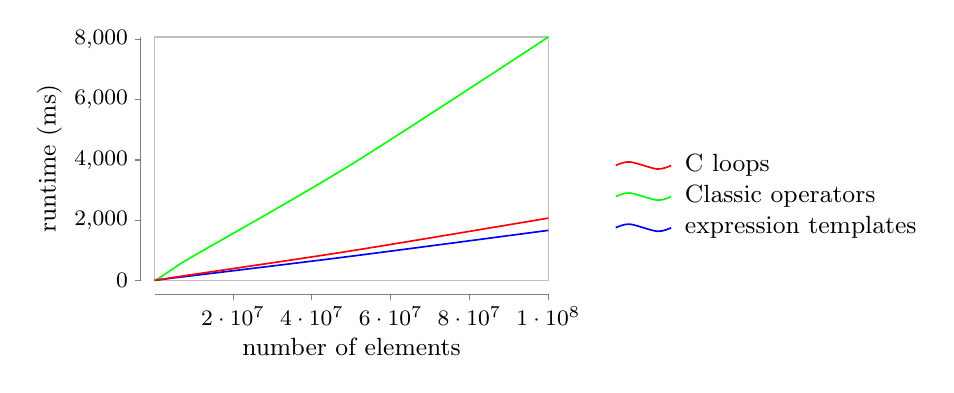
\begin{tikzpicture}
        \datavisualization[scientific axes=clean,
            x axis={label = {number of elements}},
            y axis={label = {runtime (ms)}},
            style sheet=strong colors,
        visualize as smooth line = cstyle,
        visualize as smooth line = classic,
        visualize as smooth line = exptemplates,
        cstyle = {style=red,label in legend={text=C loops}},
        classic={style=green,label in legend={text=Classic operators}},
        exptemplates={style=blue,label in legend={text=expression templates}}
        ]
        data[set=cstyle]{
            x,y
            1e+5,2
            5e+5,9
            1e+6,18
            5e+6,99
            1e+7,199
            5e+7,982
            1e+8,2069
        }
        data[set=exptemplates]
        {
            x,y
            1e+5,2
            5e+5,8
            1e+6,16
            5e+6,84
            1e+7,161
            5e+7,803
            1e+8,1662
        }
        data[set=classic]{
            x,y
            1e+5,4
            5e+5,27
            1e+6,55
            5e+6,405
            1e+7,812
            5e+7,3853
            1e+8,8091        
        };
    \end{tikzpicture}
\end{frame}

%%%===========================================================================


\end{document}
